\section{Ejercicio 3 (Programacion dinamica):}
La programación dinámica es otra técnica algorítmica, consiste en resolver los subproblemas de tamaños menores y dados estos resultados, generar la solución al problema original, pero la técnica aprovecha estructuras de datos(generalmente matrices) para guardar los subproblemas que ya calculamos, y si en algún momento lo tenemos que calcular de nuevo(por ejemplo si dos subproblemas del mismo tamaño necesitan del mismo subproblema de tamaño más chico) nos ahorramos el cálculo porque tenemos en la estructura la respuesta.

Principio de optimalidad de Bellman:
Para que el problema satisfaga el principio una subsolución óptima debe ser solución del subproblema asociado a esa subsolucion. En este problema podríamos decir que para una secuencia de largo en un subproblema sea la subsecuencia de 0 a n - 1, y si tenemos esta su subsolución, entonces, la solución al problema original va a ser menor o igual a esta subsolución, de hecho va a ser igual o la misma menos uno(siempre y cuando no sea 0). Probemos esto que acabamos de decir, supongamos que tenemos una subsolucion que vale $x \geq 2$ para el subproblema de tamaño igual menos uno a la del problema que tenemos que resolver, y también supongamos que la solución al problema es un $x'$ tal que $x' = x - 2$, si pasa esto podríamos quedarnos con esa combinación de colores(con la que nos da $x'$) sacarle el último número y tendríamos una nueva subsolucion $x''$ tal que $x'' = x'-1$ ya que solamente sacamos el último número, pero entonces $x'' < x$ osea que $x$ no era óptima, por ende entramos en un absurdo. Lo absurdo sale de suponer que había una solución mucho mejor que la de la solución. Osea que de una sub solucion no podemos empeorar la solucion o solo la empeoramos en una unidad, la dejamos igual cuando el nuevo número lo podemos pintar desde alguna de la combinaciones óptimas anteriores, o empeora en uno si no existe combinación óptima anterior desde la cual no podamos pintar este numero de rojo o de azul(notar que ahora hay combinaciones que por ahí no son óptimas para el subproblema anterior pero se diferencian en uno). Gracias a esto cumple el principio de optimalidad de Bellman, pero notemos que si el problema fuese dar las subsecuencias rojas y azules, no se cumpliria el principio ya que, por lo último que dijimos, cuando no hay una combinación óptima anterior puede ser que las nuevas soluciones no están asociadas a las del subproblema, entonces no cumpliria el principio.

Como vimos en backtracking al pintar un numero, solo nos importa cuales fueron el último rojo y el último azul que se pintaron, entonces al agregar un nuevo número a la secuencia, tenemos que buscar la combinación del último rojo y último azul óptima tal que nos deje pintar este último número o buscar una combinación de rojo y azul la cual no pintemos este último pero sea mejor que si lo pintamos. Entonces por problema tenemos que buscar cual es la combinación de último rojo y último azul que nos haga óptima la solución.

El algoritmo dado se va a basar en eso, va a terminar calculando todas las combinaciones de último rojo y último azul para ver cual es la óptima. Como calculamos cada una de estas combinaciones? recientemente dijimos que para pintar un número de forma óptima teníamos que buscar en la combinación de ultimo rojo ultimo azul valida que sea óptima. Entonces si queremos pintar el último índice de rojo, sea $r$, y como último azul un índice $a$ con $0 \leq a < r$, deberíamos buscar el $r'$ tal que sea óptimo y qué $secuencia_{r'} < secuencia_r$, para esto vamos a tener que recorrer de $0$ a $r-1$ buscando el que cumpla estas condiciones.
Otro tema importante de la programación dinámica es como guardamos los datos, una manera es tener una matriz de 2 dimensiones, en el que el índice de la fila representa el índice del último azul y el índice de la columnas el del rojo, osea que sea $M$ la matriz, $M_{r,b}$ nos da cual la sub solucion para esa combinación de rojo y azul. Un caso que deje afuera pero hay que tener en cuenta es que hay una combinación que es en la que no se pinta ninguno de rojo o de azul, o no se pinta ninguno, este índice se va a representar en la última fila y en la última columna, resumiendo para un problema de $n$ números vamos a tener una matriz $M$ de ($n+1 x n+1$) donde la la fila n+1 y la columna n+1 representan cuando el último azul o ultimo rojo respectivamente son nulos.

Este es nuestro algoritmo, calculamos la matriz y buscamos en ella cuál es el óptimo, ahora tenemos que decidir en qué orden calculamos los datos, ya que como para calcular $M_{r,b}$ tenemos que tener calculado $M_{i,b}$ con $i<r$ y $M_{r+1,b}$ va a necesitar de estos también, podemos ir de una manera constructiva, empezando en los casos bases, que son los cuando pintamos nada más el primero de un color(que sabemos que va a dejar a todos los otros números siguientes sin pintar entonces la subsolución es n - 1) y si no pintamos ninguno(osea quedan n sin pintar), esto era el índice 0, después pasamos para el índice 1 y calculamos todas las combinaciones nuevas, osea ya teníamos calculado $M_{0,n+1}$ y $M_{n+1,0}$ y $M_{n+1,n+1}$, y ahora calculamos $M_{1,0}$, $M_{1,n+1}$, $M_{0,1}$, $M_{n+1, 1}$ (notar que $M_{r,b}$ con $r = b$ es inválido porque no podemos pintar un mismo número de dos colores). Una vez calculada toda la matriz buscamos el óptimo dentro de esta y esa es nuestra solución.\\

\begin{algorithm}[H]
\NoCaptionOfAlgo
	\KwData{	
	arreglo = el arreglo de numeros entero\\
	n = el tamaño del arreglo\\
	\KwResult{La cantidad minima de numeros sin pintar para una secuencia de numeros de largo n}
	\caption{\algoritmo{ej3}{int arreglo[], n}{int}}
		\tcc{Creamos nuestra matriz}
		int m[n+1][n+1]\\ \\

		\tcc{Le guardamos los triviales, los del primer indice(0)}
		int m[0][n] = n - 1\\
		int m[n][0] = n - 1\\
		int m[n][n] = n \\ \\

		\tcc{Ahora recorremos todos los indices}
		\For(){$i \leftarrow 1$ \KwTo n}{
			\tcc{Y para cada indice, calculamos el optimo si pintaramos este de azul o de rojo y las combinaciones del otro}
			\For(){$j \leftarrow o$ \KwTo i - 1}{
				m[i][j] $\leftarrow$ buscarOptimoPintandoDeRojo(i, j, arreglo, m, n) \\
				m[j][i] $\leftarrow$ buscarOptimoPintandoDeAzul(i, j, arreglo, m, n)
			}
			\\
			\tcc{En esa iteracion dejamos de lado la combinacion si pintamos este ultimo de azul y no pintamos ninguno de rojo, y viceversa}
			m[i][n] $\leftarrow$ buscarOptimoPintandoDeRojo(i, n, arreglo, m, n) \\
			m[n][i] $\leftarrow$ buscarOptimoPintandoDeAzul(i, n, arreglo, m, n)
		}

		\tcc{Una vez ya calculada la matriz buscamos el menor, min es una funcion que busca el menor de una matriz en $O(m)$ donde m es la cantidad de elementos que hay en la matriz}
		res $\leftarrow$ min(m)
	}
\end{algorithm}
.\\
\begin{algorithm}[H]
\NoCaptionOfAlgo
	\KwData{	
	r = El indice que estamos pintando de rojo\\
	a = El indice que fijamos de azul\\
	arreglo = La secuencia de numeros \\
	m = La matriz(pasa por referencia)\\
	n = el tamaño del arreglo\\
	\KwResult{La cantidad minima de numeros sin pintar si elejimos como ultimo pintado de rojo al indice r y de azul a a}
	\caption{\algoritmo{buscarOptimoPintandoDeRojo}{int r, a, arreglo[], m, n}{int}}
		\tcc{Ponemos como optimo momentaneo al $M_{n, a}$ osea si el primer rojo que pintamos sea este numero, total siempre es una solucion valida}
		int optimoActual $\leftarrow$ m[n][a]\\
		\tcc{Recorremos con el azul fijado, que pasaria si partieramos desde los anteriores rojos}
		\For(){$ri \leftarrow 0$ \KwTo r - 1}{
			\tcc{Nos fijamos si el numero de la secuencia de ri es menor al de r,(osea si podemos pintarlo a partir de ri), y si es mas chico que el optimoActual}
			\If{ri != a \textbf{and} arreglo[ri] $<$ arreglo[r] \textbf{and} m[ri][a] $<$ optimoActual}{
				\tcc{Si es menor, marcamos a este como el optimoActual}
				optimoActual $\leftarrow$ m[ri][a]
			}
		}
		\tcc{Retornamos el optimo del cual podemos pintar y como pintamos este ultimo se reduce en 1}
		res $\leftarrow$ optimoActual - 1 
	}
\end{algorithm}

\begin{algorithm}[H]
\NoCaptionOfAlgo
	\KwData{	
	a = El indice que estamos pintando de azul\\
	r = El indice que fijamos de rojo\\
	\caption{\algoritmo{buscarOptimoPintandoDeRojo}{int a, j, arreglo[], m, n}{int}}
		\tcc{El codigo de esta funcion es totalmente analogo al de rojo}
		int optimoActual $\leftarrow$ m[r][n]\\
		\For(){$ai \leftarrow 0$ \KwTo a - 1}{
			\If{ai != r \textbf{and} arreglo[ai] $>$ arreglo[a] \textbf{and} m[r][ai] $<$ optimoActual}{
				optimoActual $\leftarrow$ m[r][ai]
			}
		}
		res $\leftarrow$ optimoActual - 1 
	}
\end{algorithm}

\subsection*{Analisis de Complejidad}
Vamos a calcular en todos los casos, toda la matriz que ambas dimensiones son de tamaños $n+1$, osea que ya recorrer todos los elementos nos cuesta $O(n^2)$ y para calcular cada una de estos elementos de la matriz recorremos $O(n)$ elementos(en la función auxiliar para buscar el óptimo), eso ya nos da una complejidad de $O(n^3)$ y después buscar el óptimo dentro de la matriz también es $O(n^2)$ y después son una cantidad constante de operaciones elementales, en definitiva nos queda una complejidad para el peor de los casos de $O(n^3)$, de hecho en el código dado no cortamos nunca y siempre completamos la matriz entonces para cualquier caso el código va a hacer $O(n^3)$. Una alternativa de análisis es considerar los casos que tenemos, podríamos decir que tenemos 3 variables en cada caso, el último azul, el ultimo rojo, y el índice, entonces como cada una de estas variables está acotada por $n$ tenemos $n^3$ casos y son los que terminamos calculando.


\subsection*{Experimentación Computacional}
\subsubsection*{Instancias Aleatorias}
De vuelta usamos las mismas instancias que antes, generadas para el ejercicio 1.

\begin{center}
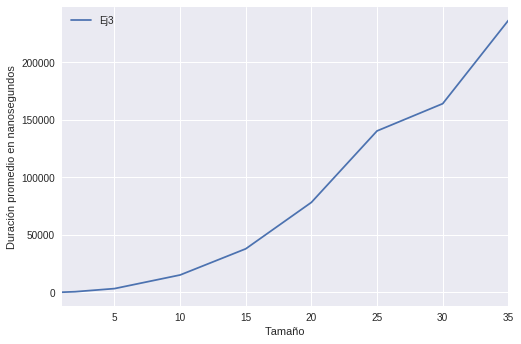
\includegraphics[scale=0.5]{ej3Random1-40.png}\\
\end{center}
Ya a simple vista podemos ver que no crece exponencialmente si no mas lineal, compramoslo con los otros ejercicios
\begin{center}
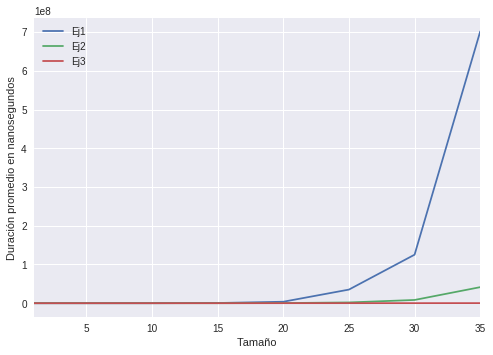
\includegraphics[scale=0.5]{ej123.png}\\
\end{center}
Obviamente no es que se mantiene constante, es que es mucho menor y a esa escala no se puede apreciar que va aumentando. El segundo ejercicio tarda 0,041461628 segundos y este tarda 0,236551 milisegundos la diferencia es abismal. Aqui podemos notar la diferencia entre un algoritmo exponencial vs uno polimonial donde para instancias grande el exponencial ya es muy grande.





